\documentclass{training}
% Filigrane PAR MODULE : \uxfond (PNG A4 dilue 30 %). Cadre noir vectoriel commun.
% Proportions original 744 px : marge 20/744, trait 1/744. Exterieur BLANC.
% Cadre via eso-pic +\put (coordonnees absolues) — pas de remember picture (decalage).
\usepackage{eso-pic}

\providecommand{\uxfond}{../../resources/fond/norme_fond_paliers_30.png}

\newlength{\uxmargin}
\newlength{\uxthick}
\newlength{\uxinnerw}
\newlength{\uxinnerh}
\setlength{\uxmargin}{0.02688\paperwidth}% 20/744
\setlength{\uxthick}{0.001344\paperwidth}% 1/744
\setlength{\uxinnerw}{\dimexpr\paperwidth-2\uxmargin-2\uxthick\relax}
\setlength{\uxinnerh}{\dimexpr\paperheight-2\uxmargin-2\uxthick\relax}

% Contenu strictement a l'interieur du trait (+ jour confortable).
\geometry{%
  includeheadfoot,
  left=22mm,
  right=22mm,
  top=20mm,
  bottom=18mm,
  headheight=30pt,
  headsep=5mm,
  footskip=12mm%
}

\AddToShipoutPictureBG{%
  \AtPageLowerLeft{%
    % Fond blanc page entiere
    \put(0,0){\color{white}\rule{\paperwidth}{\paperheight}}%
    % Filigrane module a l'interieur du cadre
    \put(\LenToUnit{\dimexpr\uxmargin+\uxthick\relax},\LenToUnit{\dimexpr\uxmargin+\uxthick\relax}){%
      \includegraphics[width=\uxinnerw,height=\uxinnerh]{\uxfond}}%
    % Cadre noir : bas, haut, gauche, droite
    \put(\LenToUnit{\uxmargin},\LenToUnit{\uxmargin}){%
      \color{black}\rule{\dimexpr\paperwidth-2\uxmargin\relax}{\uxthick}}%
    \put(\LenToUnit{\uxmargin},\LenToUnit{\dimexpr\paperheight-\uxmargin-\uxthick\relax}){%
      \color{black}\rule{\dimexpr\paperwidth-2\uxmargin\relax}{\uxthick}}%
    \put(\LenToUnit{\uxmargin},\LenToUnit{\uxmargin}){%
      \color{black}\rule{\uxthick}{\dimexpr\paperheight-2\uxmargin\relax}}%
    \put(\LenToUnit{\dimexpr\paperwidth-\uxmargin-\uxthick\relax},\LenToUnit{\uxmargin}){%
      \color{black}\rule{\uxthick}{\dimexpr\paperheight-2\uxmargin\relax}}%
  }%
}

\makeatletter
\fancyhf{}
\fancyheadoffset{0pt}
\renewcommand{\headrulewidth}{0pt}
\lhead{\parbox[t]{0.56\textwidth}{\RaggedRight\footnotesize\sloppy\@title}}
\rhead{\parbox[t]{0.36\textwidth}{\RaggedLeft\footnotesize\sloppy\@subtitle}}
\cfoot{\thepage}
% Coupures : underscore et slash dans les noms de fichiers / consignes
\DeclareRobustCommand{\_}{\textunderscore\allowbreak}
\makeatother

% Evite les depassements de longues lignes (Github, Name_FirstName_...)
\sloppy
\emergencystretch=3em
\hbadness=10000

% Sommaire type 42 : chapitres seulement
\setcounter{tocdepth}{0}
\renewcommand{\cftchappresnum}{}
\renewcommand{\cftchapaftersnum}{}
\setlength{\cftchapnumwidth}{2.0em}
\setlength{\cftbeforechapskip}{0.35em}
\cftsetindents{chapter}{0em}{2.0em}


\begin{document}

\schoollogo{../../resources/jeunecrack.png}
\title{Sunday night movie}
\subtitle{Piscine UX/UI --- UX}
\member{Piscine UX/UI}{https://github.com/01-edu/UX-UI}
\summary{A flow, wireframes, motion, three feature tests, one iteration.}
\version{1.0}
\prerequisite{The previous module of this piscine, or none if this is your first.}
\maketitle

\newpage
\tableofcontents
\newpage


\chapter{Instructions}

The foreword is not an exercise. It will not be graded. The exercises start at the next chapter, from the easiest contract to the hardest. A later exercise is not taken into account if an earlier one does not hold.

Only what is in the turn-in directory of an exercise is looked at. Do not add files that the exercise does not name. The name of a deliverable follows the pattern in the exercise: \texttt{Name\_FirstName\_DeliverableName\_Date\_VersionNumber}.

You will not be given the gesture. The examples in an exercise sometimes carry a constraint that the sentence does not repeat. Read them. Your other references are the manual of the tool you picked, the person sitting next to you, and the links printed in the exercise.

The order is the order of the quest. Skipping a step because a later screen looks more interesting produces a screen nobody can explain.

\subsection*{About the pictures}

The mark on the cover is the project logo. The picture in the foreword is the illustration of this module. The pale ground behind the text is the page watermark. None of them is a hint.

\subsection*{About machines that write}

You may use a tool to look up a term, the way you would use a dictionary. You may not replace an interview, a test, or a file with a generated text and sign it. If you cannot point at the person, the screen, or the line you claim, the exercise is not done.


\chapter{Foreword}

Saul Bass made the titles of a film do the work of a first scene (\emph{Anatomy of a Murder}, 1959, is the usual example). A Sunday night in front of a screen has the same contract: the first minute must tell you where you are. The exercises ask you to draw that minute and then watch someone miss it.

\begin{center}
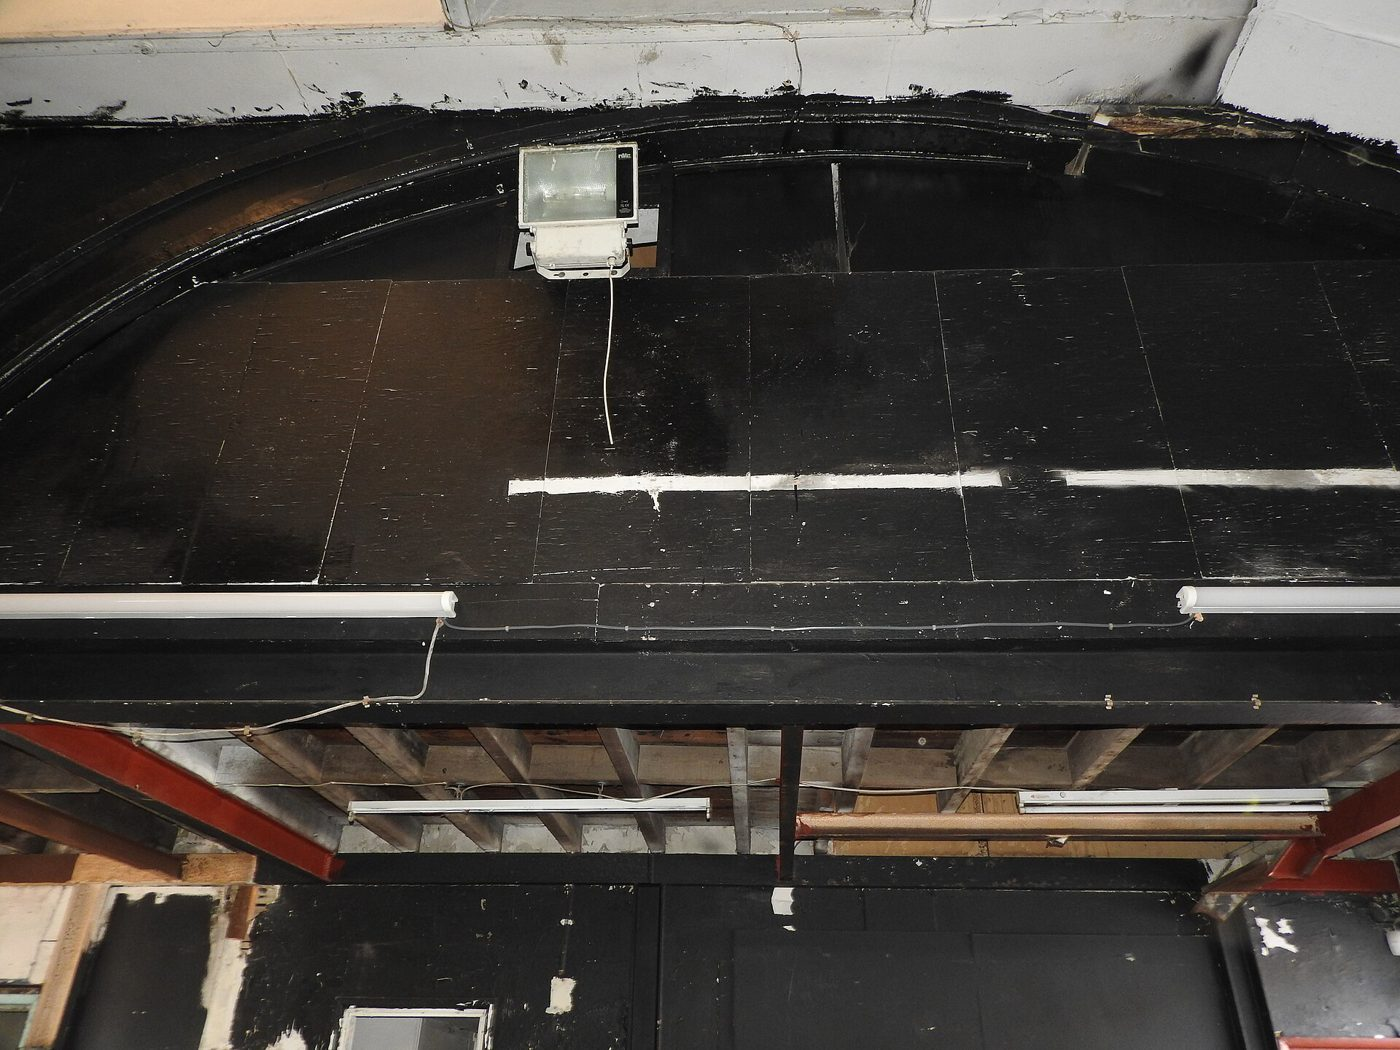
\includegraphics[width=0.78\textwidth,height=0.32\textheight,keepaspectratio]{../../resources/intros/UX-05-sunday-night-movie.jpg}\\[0.4em]
{\footnotesize Picture: ClemRutter / CC BY-SA 4.0}
\end{center}

Recommended watching. The videos are context. They are not the deliverable.
\begin{itemize}
\item UX - Introduction \& Quest n°1, 01Edu \url{https://www.youtube.com/watch?v=UbE6WMeuvQg&list=PLHyAJ_GrRtf-RAtfngbRrFh1XDTnyXFDe}
\end{itemize}

\chapter{Exercise 00: UX VI - Ex 1 - User flow}
\exnumber{00}
\extitle{UX VI - Ex 1 - User flow}
\exfiles{ex00/Figma file, named Name\_FirstName\_DeliverableName\_Date\_VersionNumber}
\exauthorize{Those named in the exercise}
\makeheaderfiles

\textbf{Context:}

Your company's client is a movie theaters chain called, Movie 4 all.

They want to launch a platform for people who want to watch movies but don't want to spend endless time selecting one.
You are replacing someone in the company who has already worked on the user research, the problem statement and the list of features they plan to develop. Your goal is to prototype and test these features.

\textbf{Instructions:}

Based on the 3 features that have come out of the ideation workshops led by your collegues, design 3 user flows (1 per feature).

Features:

\begin{itemize}
\item 1: Adding a filter based on their current mood
\item 2: Offer a selection of 3 movies to be watched
\item 3: Ask users to rate the movie after watching it for further recommendation
\end{itemize}

\textbf{Deliverables:}

\begin{itemize}
\item 3 user flows on a board (digital or pictures of a paper board)
\item Upload the documents on Github, in a zip folder named "ProjectTitle\_Name\_FirstName", with all project deliverables as follows: "Name\_FirstName\_DeliverableName\_Date\_VersionNumber".  For example, the first deliverable can be named as "Doe\_John\_MidFiPrototype\_05242024\_V1".
\item Add a title within all written documents.
\item Pay attention to the global aspect of the deliverables. They must be clear, simple and easy to read. You can get inspiration on canva.com but don't overload your design with too much details!
\end{itemize}

\textbf{Resources:}

\begin{itemize}
\item User flow glossary \url{https://www.productplan.com/glossary/user-flow/}
\item Site flows vs User Flows \url{https://uxmovement.com/wireframes/site-flows-vs-user-flows-when-to-use-which/}
\item How to make a User Flow diagram \url{https://www.lucidchart.com/blog/how-to-make-a-user-flow-diagram}
\end{itemize}

\textbf{Recommended tools:}

\begin{itemize}
\item Figma
\item Whimsical
\end{itemize}


\chapter{Exercise 01: UX VI - Ex 2 - Wireframes}
\exnumber{01}
\extitle{UX VI - Ex 2 - Wireframes}
\exfiles{ex01/Figma file, named Name\_FirstName\_DeliverableName\_Date\_VersionNumber}
\exauthorize{Those named in the exercise}
\makeheaderfiles

\textbf{Instructions:}

Based on the 3 user flows, design 3 series of wireframes.

\textbf{Deliverables:}

\begin{itemize}
\item 3 series of wireframes (6 to 12 screens per flow) on Figma
\item Upload the documents on Github, in a zip folder named "ProjectTitle\_Name\_FirstName", with all project deliverables as follows: "Name\_FirstName\_DeliverableName\_Date\_VersionNumber".  For example, the first deliverable can be named as "Doe\_John\_MidFiPrototype\_05242024\_V1".
\item Pay attention to the global aspect of the deliverables. They must be clear, simple and easy to read. You can get inspiration on canva.com but don't overload your design with too much details!
\end{itemize}

\textbf{Tips:}

\begin{itemize}
\item Drawing paper prototypes before going digital might save you some time ;)
\item Vocabulary
\begin{itemize}
\item Low-Fidelity: Paper Prototypes - Example here \url{https://miro.medium.com/max/1400/1*5nUfqqA2gjdAYHagjbHA5w.jpeg}
\item Mid-Fidelity: Wireframes - black and white, only the main elements, on digital prototype tools - Example here \url{https://miro.medium.com/max/1400/1*eGSfaxwYbxUFomYbyO6GWw.png}
\item High-Fidelity: Wireframes with color, styles, graphical details, and micro-interactions - Example here \url{https://miro.medium.com/max/1400/1*Xn0HSKAvhr4TZzC9lN5udw.gif}
\end{itemize}
\end{itemize}

\textbf{Resources:}

\begin{itemize}
\item How to start sketching and wireframing \url{https://uxdesign.cc/how-to-start-sketching-and-wireframing-84a821f092e2}
\item Why should product teams use wireframes more often? \url{https://uxdesign.cc/why-should-product-teams-use-wireframes-more-often-60e34a2bc55}
\item The 5-pass reduction wireframing: A minimalist UX technique \url{https://uxdesign.cc/the-5-pass-reduction-wireframing-a-minimalist-ux-technique-aa415aad9ce2?sk=a218ac4db9d1049249bd381fbc5edeee}
\item The art of designing good wireframes \url{https://uxdesign.cc/the-art-of-designing-good-wireframes-8a2a9c10a95b}
\end{itemize}

\textbf{Recommended tools:}

\begin{itemize}
\item Figma
\end{itemize}

\textbf{Quote:}

'77\% of users return to content and information sites because of ease-of-use. Only 22\% return because the site belongs to a favorite brand.' Forrester


\chapter{Exercise 02: UX VI - Ex 3 - Wireframes animation}
\exnumber{02}
\extitle{UX VI - Ex 3 - Wireframes animation}
\exfiles{ex02/Figma file, named Name\_FirstName\_DeliverableName\_Date\_VersionNumber}
\exauthorize{Those named in the exercise}
\makeheaderfiles

\textbf{Instructions:}

Animate your wireframes on Figma.

Think about multistate!!

This exercise is to be made individually.

\textbf{Deliverables:}

\begin{itemize}
\item An animated prototype on Figma
\item Upload the Figma file on Github, labeled as follows: "Name\_FirstName\_DeliverableName\_Date\_VersionNumber". For example, it can be labeled as "Doe\_John\_MidFiPrototype\_05242024\_V1".
\item Add a title within the file.
\item Pay attention to the global aspect of the file. It must be clear, simple and easy to read. You can get inspiration on canva.com but don't overload your design with too much details!
\end{itemize}

\textbf{Resources:}

\begin{itemize}
\item Efficiently Manage Your Designs - How Mockplus State Page Helps To View \& Manage Multiple State \url{https://help.mockplus.com/p/372}
\end{itemize}


\chapter{Exercise 03: UX VI - Ex 4 - Test on feature \#1}
\exnumber{03}
\extitle{UX VI - Ex 4 - Test on feature \#1}
\exfiles{ex03/zip archive, named Name\_FirstName\_DeliverableName\_Date\_VersionNumber}
\exauthorize{Those named in the exercise}
\makeheaderfiles

\textbf{Instructions:}

Test your wireframes!

Focus on the 1st journey. Prepare a test protocol with your research goals (what you want to test), test it on 5 different people and write down 3 ways to improve the prototype.

\textbf{Deliverables:}

\begin{itemize}
\item A PDF document with a Test protocol
\item Pictures of the ongoing tests
\item A PDF document with 3 ideas to improve the prototype based on you users' feedbacks.
\item Upload the documents on Github, in a zip folder named "ProjectTitle\_Name\_FirstName", with all project deliverables as follows: "Name\_FirstName\_DeliverableName\_Date\_VersionNumber".  For example, the first deliverable can be named as "Doe\_John\_MidFiPrototype\_05242024\_V1".
\item Add a title within all written documents.
\item Pay attention to the global aspect of the deliverables. They must be clear, simple and easy to read. You can get inspiration on canva.com but don't overload your design with too much details!
\end{itemize}

\textbf{Resources:}

\begin{itemize}
\item How to do a user interview (tutorial from Google Ventures) \url{https://www.youtube.com/watch?v=Qq3OiHQ-HCU}
\item Running a usability test \url{https://www.usability.gov/how-to-and-tools/methods/running-usability-tests.html}
\item Usability testing: what is it and how to do it? \url{https://uxdesign.cc/usability-testing-what-is-it-how-to-do-it-51356e5de5d}
\item Analyzing usability testing data \url{https://uxdesign.cc/analysing-usability-testing-data-97667ae4999e}
\item The art of guerrilla usability testing \url{http://www.uxbooth.com/articles/the-art-of-guerrilla-usability-testing/}
\item How to write a user testing report that people will actually read \url{https://uxdesign.cc/how-to-write-a-user-testing-report-that-people-will-actually-read-652d15d2f92e}
\end{itemize}


\chapter{Exercise 04: UX VI - Ex 5 - Test on feature \#2}
\exnumber{04}
\extitle{UX VI - Ex 5 - Test on feature \#2}
\exfiles{ex04/zip archive, named Name\_FirstName\_DeliverableName\_Date\_VersionNumber}
\exauthorize{Those named in the exercise}
\makeheaderfiles

\textbf{Instructions:}

Test your wireframes!

Focus on the 2nd journey. Prepare a test protocol with your research goals (what you want to test), test it on 5 different people and write down 3 ways to improve the prototype.

\textbf{Deliverables:}

\begin{itemize}
\item A PDF document with a Test protocol
\item Pictures of the ongoing tests
\item A PDF document with 3 ideas to improve the prototype based on you users' feedbacks.
\item Upload the documents on Github, in a zip folder named "ProjectTitle\_Name\_FirstName", with all project deliverables as follows: "Name\_FirstName\_DeliverableName\_Date\_VersionNumber".  For example, the first deliverable can be named as "Doe\_John\_MidFiPrototype\_05242024\_V1".
\item Add a title within all written documents.
\item Pay attention to the global aspect of the deliverables. They must be clear, simple and easy to read. You can get inspiration on canva.com but don't overload your design with too much details!
\end{itemize}

\textbf{Resources:}

\begin{itemize}
\item How to do a user interview (tutorial from Google Ventures) \url{https://www.youtube.com/watch?v=Qq3OiHQ-HCU}
\item Running a usability test \url{https://www.usability.gov/how-to-and-tools/methods/running-usability-tests.html}
\item Usability testing: what is it and how to do it? \url{https://uxdesign.cc/usability-testing-what-is-it-how-to-do-it-51356e5de5d}
\item Analyzing usability testing data \url{https://uxdesign.cc/analysing-usability-testing-data-97667ae4999e}
\item The art of guerrilla usability testing \url{http://www.uxbooth.com/articles/the-art-of-guerrilla-usability-testing/}
\item How to write a user testing report that people will actually read \url{https://uxdesign.cc/how-to-write-a-user-testing-report-that-people-will-actually-read-652d15d2f92e}
\end{itemize}


\chapter{Exercise 05: UX VI - Ex 6 - Test on feature \#3}
\exnumber{05}
\extitle{UX VI - Ex 6 - Test on feature \#3}
\exfiles{ex05/zip archive, named Name\_FirstName\_DeliverableName\_Date\_VersionNumber}
\exauthorize{Those named in the exercise}
\makeheaderfiles

\textbf{Instructions:}

Test your wireframes!

Focus on the 3rd journey. Prepare a test protocol with your research goals (what you want to test), test it on 5 different people and write down 3 ways to improve the prototype.

\textbf{Deliverables}:

\begin{itemize}
\item A PDF document with a Test protocol
\item Pictures of the ongoing tests
\item A PDF document with 3 ideas to improve the prototype based on you users' feedbacks.
\item Upload the documents on Github, in a zip folder named "ProjectTitle\_Name\_FirstName", with all project deliverables as follows: "Name\_FirstName\_DeliverableName\_Date\_VersionNumber".  For example, the first deliverable can be named as "Doe\_John\_MidFiPrototype\_05242024\_V1".
\item Add a title within all written documents.
\item Pay attention to the global aspect of the deliverables. They must be clear, simple and easy to read. You can get inspiration on canva.com but don't overload your design with too much details!
\end{itemize}

\textbf{Resources}:

\begin{itemize}
\item How to do a user interview (tutorial from Google Ventures) \url{https://www.youtube.com/watch?v=Qq3OiHQ-HCU}
\item Running a usability test \url{https://www.usability.gov/how-to-and-tools/methods/running-usability-tests.html}
\item Usability testing: what is it and how to do it? \url{https://uxdesign.cc/usability-testing-what-is-it-how-to-do-it-51356e5de5d}
\item Analyzing usability testing data \url{https://uxdesign.cc/analysing-usability-testing-data-97667ae4999e}
\item The art of guerrilla usability testing \url{http://www.uxbooth.com/articles/the-art-of-guerrilla-usability-testing/}
\item How to write a user testing report that people will actually read \url{https://uxdesign.cc/how-to-write-a-user-testing-report-that-people-will-actually-read-652d15d2f92e}
\end{itemize}


\chapter{Exercise 06: UX VI - Ex 7 - Iteration}
\exnumber{06}
\extitle{UX VI - Ex 7 - Iteration}
\exfiles{ex06/zip archive, named Name\_FirstName\_DeliverableName\_Date\_VersionNumber}
\exauthorize{Those named in the exercise}
\makeheaderfiles

\textbf{Instructions:}

Based on your previous tests, pick one of your 3 prototypes.

Implement the 3 ideas you wrote down as suggestions.

Run another series of test (and adapt your test protocol if necessary).

Write a report with the conclusion you made out of this iteration loop.

\textbf{Deliverables:}

\begin{itemize}
\item Pictures of the new test
\item A report with your conclusions, your impressions and your key learnings from this iteration (PDF document out of Microsoft Word, Pages, Google Docs or any word-processing software)
\item Comparison between V1 and V2 of the prototype in the report
\item Upload the documents on Github, in a zip folder named "ProjectTitle\_Name\_FirstName", with all project deliverables as follows: "Name\_FirstName\_DeliverableName\_Date\_VersionNumber".  For example, the first deliverable can be named as "Doe\_John\_MidFiPrototype\_05242024\_V1".
\item Add a title within all written documents.
\item Pay attention to the global aspect of the deliverables. They must be clear, simple and easy to read. You can get inspiration on canva.com but don't overload your design with too much details!
\end{itemize}

\textbf{Tips:}

\begin{itemize}
\item This report will be handed on to the CEO. Pay attention to the details and make sure the document is clean and easy to use!
\end{itemize}


\end{document}
